

\chapter{Systemanalyse}
\section{Systemkontextdiagramm}



\begin{figure}[H]
	\begin{tikzpicture}[node distance=5]
		\node [draw, rectangle, drop shadow, fill=white] (F) {Fahrzeug};
		\node [draw, circle, drop shadow, fill=white, text width=3cm, align=center] (C) [below right=of F] {MEC-Server};
		\node [draw, rectangle, drop shadow, fill=white] (S) [below right=of C] {Sensor};
		\node [draw, rectangle, drop shadow, fill=white] (A) [above right=of C] {Fusions-Algorithmus};
		
		\node (ctrl1) [above=of S] {};
		\node (ctrl2) [above right=of C] {};
		\node (ctrl3) [right=of C] {};
	%	\node (ctrl4) [above right=of S] {};
		\node (ctrl5) [left=of C] {};
		\node (ctrl6) [below=of ctrl5] {};
		
		%
		% Fahrzeug -> MEC-Server
		%
		\path[draw, -{Latex[scale=2.0]}, dashed] (F)
				edge [bend right] node [fill=white] {GeoFence verlassen} (C)
				edge [bend left]  node [fill=white] {GeoFence betreten} (C);
				
		%
		% MEC-Server -> Fahrzeug
		%
		\path[draw, -{Latex[scale=2.0]}] (C)
				edge node [fill=white] {Fusions-Algorithmus Ergebnis} (F);
				
		%
		% MEC-Server -> Algorithmus
		%
		\path[draw, -{Latex[scale=2.0]}] (C)
				edge [bend right] node [fill=white] {Sensordaten} (A);
		
		%
		% Algorithmus -> MEC-Server
		%
		\path[draw, -{Latex[scale=2.0]}] (A)
				edge [bend right] node [fill=white] {Ergebnis} (C);
		
		%
		% Sensor -> MEC-Server
		%		
		\path[draw, -{Latex[scale=2.0]}, dashed] (S)
			edge [bend left]  node [fill=white] {GeoFence betreten} (C);
		\path[draw, -{Latex[scale=2.0]}] (S)
			edge node [fill=white] {Sensordaten} (C);
				
		%
		% MEC-Server -> Fahrzeug
		%
		\path[draw, -{Latex[scale=2.0]}, dashed] (C)
			edge [bend left] node [fill=white] {Wecken} (S)
			.. controls (ctrl1) and (ctrl3) ..  node [fill=white] {Pausieren} (S);
				
				
		
		\path[draw, -{Latex[scale=2.0]}] (4, -8) -- (.5, -8) node [pos=.5, above] {Datenfluss};
		\path[draw, -{Latex[scale=2.0]}, dashed] (4, -9) -- (.5, -9) node [pos=.5, above] {Kontrollfluss};
			
	\end{tikzpicture}
	\centering
	\label{system_context}
	\caption{Systemkontextdiagramm}
\end{figure}

\section{Komponentendiagramm oder sowas?}
\section{Use Case Diagramme}
\todo{was wirklich umgesetzt sein wird}

\begin{figure}[H]
	\begin{tikzpicture}[node distance=5]
		\begin{umlsystem}{MEC-Server}
			\umlusecase[y=4,name=u0]{Verbindung aufbauen}
			\umlusecase[y=2,name=u1]{GeoFence betreten}
			\umlusecase[y=0,name=u2]{GeoFence verlassen}
			\umlusecase[y=-2,name=u3]{Sensordaten senden}
			\umlusecase[y=-4,name=u4]{Umfeldmodel übergeben}
		\end{umlsystem}
		\umlactor[x=-6,y=2]{Fahrzeug}
		\umlactor[x=-6,y=-4]{Fusions-Algorithmus}
		\umlactor[x=6,y=1]{Sensor}
		\umlassoc{Fahrzeug}{u0}
		\umlassoc{Fahrzeug}{u1}
		\umlassoc{Fahrzeug}{u2}
		\umlassoc{Sensor}{u0}
		\umlassoc{Sensor}{u1}
		\umlassoc{Sensor}{u3}
		\umlassoc{Fusions-Algorithmus}{u4}
	\end{tikzpicture}
	\centering
	\label{use_case:car}
	\caption{Use Case Diagramm für den MEC-Server}
\end{figure}


\begin{figure}[H]
	\begin{tikzpicture}[node distance=5]
		\begin{umlsystem}{Sensor}
			\umlusecase[y=0,name=u1]{Pausieren}
			\umlusecase[y=2,name=u2]{Wecken}
		\end{umlsystem} 
		\umlactor[x=-3.5,y=1]{MEC-Server}
		\umlassoc{MEC-Server}{u1}
		\umlassoc{MEC-Server}{u2} 
	\end{tikzpicture}
	\centering
	\label{use_case:server_sensor}
	\caption{Use Case Diagramm des MEC-Servers gegenüber dem Sensor}
\end{figure}

\begin{figure}[H]
	\begin{tikzpicture}[node distance=5]
		\begin{umlsystem}{Fahrzeug}
			\umlusecase[y=0,name=u1]{Umfeldmodell senden}
		\end{umlsystem} 
		\umlactor[x=-5,y=0]{MEC-Server}
		\umlassoc{MEC-Server}{u1}
	\end{tikzpicture}
	\centering
	\label{use_case:server_vehicle}
	\caption{Use Case Diagramm des MEC-Servers gegenüber dem Sensor}
\end{figure}

\begin{figure}[H]
	\begin{tikzpicture}[node distance=5]
		\begin{umlsystem}{Fusions-Algorithmus}
			\umlusecase[y=0,name=u1]{Sensordaten übergeben}
		\end{umlsystem} 
		\umlactor[x=-5,y=0]{MEC-Server}
		\umlassoc{MEC-Server}{u1}
	\end{tikzpicture}
	\centering
	\label{use_case:server_algorithmus}
	\caption{Use Case Diagramm des MEC-Servers gegenüber dem Fusions-Algorithmus}
\end{figure}


\section{Nachrichten}


\begin{wrapfigure}{R}[-1.5em]{.5\textwidth}
	\centering
	\begin{bytefield}[bitwidth=.45em,bitheight=.7em]{32}
		\bitheader{0,31} \\
		
		\begin{rightwordgroup}{Kopf}
			\wordbox{4}{ASN.1 Nachrichtenlänge \textbf{$n$}} \\
			\wordbox{4}{ASN.1 Nachrichtentyp}
		\end{rightwordgroup} \\
		
		\begin{rightwordgroup}{Länge in\\\textbf{$n$} Bytes}
			\wordbox[lrt]{8}{ASN.1 Nachricht} \\
			\skippedwords \\
			\wordbox[lrb]{2}{}
		\end{rightwordgroup}
	\end{bytefield}
	\caption{ASN.1 Nachricht mit Header}
	\label{message:structure}
\end{wrapfigure}

Eine ASN.1 Nachricht wird, wie in \autoref{message:structure} zu sehen, mit  vorangestellten Kopfdaten versendet.
Diese Kopfdaten enthalten die Länge der ASN.1 Nachricht und dessen Typ, der bei der Dekodierung beim Empfängers bekannt sein muss.
Die Nachrichtenlänge und der Nachrichtentyp werden als 32-Bit lange und vorzeichenlose Ganzzahlen übermittelt und entsprechen damit dem Datentyp \rustcinline{u32} in Rust.
Sie werden als \enquote{Big-Endian} auf dem Datenstrom dargestellt.

Die Nachrichtenlänge gibt die Länge der ASN.1 Nachricht in Bytes an.

Für den Nachrichtentyp sind nur die in \autoref{message:types} gelisteten Werte gültig und werden im Anschluss erklärt.

\begin{figure}[H]
	\centering
	\begin{tabular}{r|l|l}
		Typ & ASN.1 Nachrichtentyp & Sichtweise des Servers \\
		\hline
		0 & Nicht definiert & -- \\
		1 & ClientRegistration & eingehend \\
		2 & SensorFrame & eingehend \\
		3 & EnvironmentFrame & ausgehend \\
		4 & UpdateSubscription & bidirektional \\
		5 & InitMessage & ausgehend \\
		6 & RoadClearanceFrame & ausgehend \\
		7 & SensorIdleFrame & eingehend \\
		8 & UpdateStatus & \todo{eingehend} \\
	\end{tabular}
	\caption{Gültige ASN.1 Nachrichtentypen}
	\label{message:types}
\end{figure}

\subsection{ClientRegistration}
\label{msg:client_registration}

Die ClientRegistration-Nachricht sendet der Client nach dem Verbindungsaufbau dem Server zu, um mitzuteilen, ob es sich um einen Sensor oder ein Fahrzeug handelt.

\subsection{SensorFrame}
\label{msg:sensor_frame}

Die SensorFrame-Nachricht wird vom Sensor an den Server versendet und beschreibt Objekte, die der Sensor erkannt hat.

\subsection{EnvironmentFrame}
\label{msg:environment_frame}

Die EnvironmentFrame-Nachricht wird vom Server an das Fahrzeug versendet und enthält das Ergebnis des Fusions-Algorithmus.

\subsection{UpdateSubscription}

Die UpdateSubscription-Nachricht wird vom Server an den Sensor oder vom Fahrzeug an den Server gesendet.
Der Sensor versendet bei einer Anmeldung erkannte Objekte (siehe \autoref{msg:sensor_frame}), während der Server dem Fahrzeug die Ergebnisse aus dem Fusions-Algorithmus (siehe \autoref{msg:environment_frame}) zusendet.
Bei einer Abmeldung wird das Versenden der Nachrichten eingestellt.

\subsection{InitMessage}

Die InitMessage-Nachricht wird vom Server nach einer Fahrzeuganmeldung (siehe \automark{ClientRegistration}) an das Fahrzeug gesendet und beinhaltet Koordinaten über die Sektoren, die die Sensoren beobachten.

\subsection{RoadClearanceFrame}

Die RoadClearanceFrame-Nachricht wird vom Server an das Fahrzeug versendet und kann Verkehrs-, Wetter- und andere Informationen über die Sektoren enthalten.

\subsection{SensorIdleFrame}

\todo{richtig?}
Die SensorIdleFrame-Nachricht wird vom Sensor an den Server versendet, wenn keine Objekte erkannt wurden aber das Zeitlimit für \todo{schweigen} erreicht wurde.

\subsection{UpdateStatus}

\todo{huh?}


%\begin{figure}[H]
%	\centering
%	\begin{bytefield}[bitwidth=.25em,bitheight=2em]{128}
%		\bitheader{0,32,64} \\
%		
%		\bitbox{32}{Länge $n$}
%		\bitbox{32}{Nachricht Id}
%		\bitbox{64}{ASN.1 Nachricht der Länge $n$}
%		%		\skippedbits
%		%		\bitbox[tbr]{32}{}
%	\end{bytefield}
%	\caption{Aufbau eines WebSocket-Frames \cite[28]{ieft:websockets}}
%	\label{figure:websockets:frame}
%\end{figure}
\todo{alternativ:}
\begin{figure}[H]
	\centering
	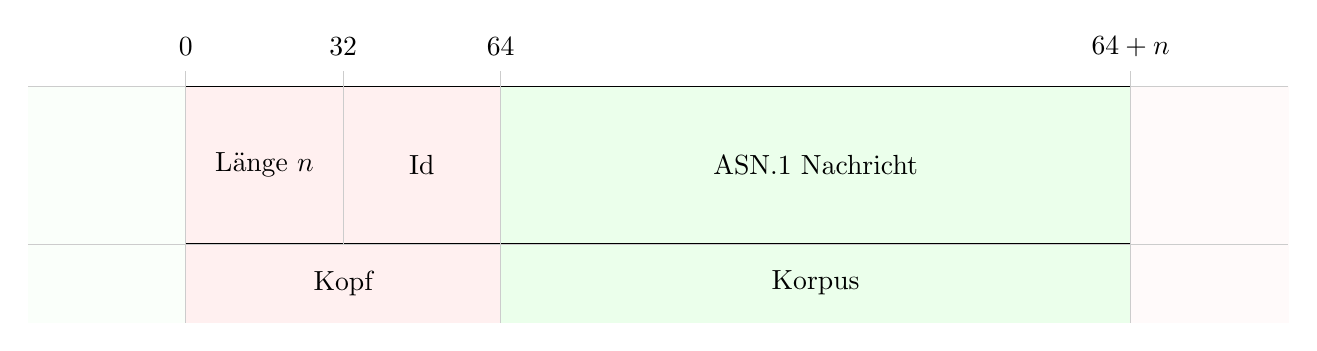
\begin{tikzpicture}
		\draw[green!2,fill] (0,0) rectangle (2,-3);
		\draw[red!6,fill] (2,0) rectangle (6,-3);
		\draw[green!8,fill] (6,0) rectangle (14,-3);
		\draw[red!2,fill] (14,0) rectangle (16,-3);
		
		\draw[gray!40, very thin] (0,0) -- (16,0);
		\draw[gray!40, very thin] (0,-2) -- (16,-2);
		\draw (2,0) -- (14,0);
		\draw (2,-2) -- (14,-2);
		\draw[gray!40, very thin] (2,-3) -- (2,0.2);
		\draw (2,0.5) node {0};
		\draw (3,-1) node {Länge $n$};
%		\draw (3,-1.7) node {\rustcinline{u32}};
		\draw[gray!40, very thin] (4,-2) -- (4,0.2);
		\draw (4,0.5) node {32};
		\draw (5,-1) node {Id};
%		\draw (5,-1.7) node {\rustcinline{u32}};
		\draw[gray!40, very thin] (6,-3) -- (6,0.2);
		\draw (6,0.5) node {64};
		\draw[gray!40, very thin] (14,-3) -- (14,0.2);
		\draw (14,0.5) node {$64 + n$};
		\draw (10,-1) node {ASN.1 Nachricht};
		
		\draw (4,-2.5) node {Kopf};
		\draw (10,-2.5) node {Korpus};
	\end{tikzpicture}
	\label{message:structure_alt}
	\caption{Aufbau einer Nachricht auf dem Datenstrom}
\end{figure}


\section{Schnitstellenanalyse}

\todo{erwartetes verhalten der sensoren und fahrzeuge}

\begin{figure}[H]
	\begin{tikzpicture}
		\begin{umlseqdiag} 
			\umlobject[x=0,class=Sensor]{c}
			\umlobject[x=11,class=MEC-Server]{s}
			\begin{umlcall}[dt=4, op={ClientRegistration\{type  = sensor, ..\}}, type=asynchron]{c}{s}
			\end{umlcall}
			\begin{umlcall}[dt=5, op={InitMessage\{..\}}, type=asynchron]{c}{s}
			\end{umlcall}
			\begin{umlfragment}[type=loop] 
				\begin{umlfragment}[type=opt, label=!paused, inner xsep=5] 
					\begin{umlcall}[dt=9, op={SensorFrame\{..\}} / SensorIdleFrame\{..\}, type=asynchron]{c}{s}
					\end{umlcall}
				\end{umlfragment}
				\begin{umlfragment}
					\begin{umlcall}[dt=9, op={UpdateSubscription\{subscription-status = unsubscribed, ..\}}, type=asynchron]{s}{c}
						\begin{umlcallself}[op={pause()}]{c}
						\end{umlcallself}
					\end{umlcall}
				\end{umlfragment}
				\begin{umlfragment}
					\begin{umlcall}[dt=9, op={UpdateSubscription\{subscription-status = subscribed, ..\}}, type=asynchron]{s}{c}
						\begin{umlcallself}[op={resume()}]{c}
						\end{umlcallself}
					\end{umlcall}
				\end{umlfragment}
			\end{umlfragment}
		\end{umlseqdiag}
	\end{tikzpicture}
	\centering
	\label{seq_dia:_}
	\caption{\todo{Sequenz Diagramm: Anmeldung und Zuweisung zu einem GeoFence eines Sensors}}
\end{figure}


\begin{figure}[H]
	\begin{tikzpicture}
		\begin{umlseqdiag} 
			\umlobject[x=0,class=Fahrzeug]{c}
			\umlobject[x=13,class=MEC-Server]{s}
			\begin{umlcall}[dt=5, op={UpdateSubscription\{subscription-status  = subscribed, ..\}}, type=asynchron]{c}{s}
			\end{umlcall}
			\begin{umlfragment}[type=loop] 
				\begin{umlfragment}[type=loop, label=!paused] 
					\begin{umlcall}[dt=5, op={ASN::Detection}, type=asynchron]{c}{s}
					\end{umlcall}
				\end{umlfragment}
				\begin{umlcall}[dt=5, op={ASN::Pause}, type=asynchron]{s}{c}
				\end{umlcall}
				\begin{umlcall}[dt=5, op={ASN::Resume}, type=asynchron]{s}{c}
				\end{umlcall}
			\end{umlfragment}
		\end{umlseqdiag}
	\end{tikzpicture}
	\centering
	\label{seq_dia:vehicle}
	\caption{\todo{Sequenz Diagramm: Anmeldung und Übermittlung an ein Fahrzeug}}
\end{figure}